\subsection{Onboarding}
%Onboarding 
The first impression you get when meeting somebody for the first time is usually a strong indicator that determines whether you will like the company of this new person or not. Similarly, the first impression or the first minutes of interacting with a game are the most important because a player will make a decision whether he or she will continue exploring the game. According to Zichermann et al. \cite{48}, the onboarding process is critical to a successful game. A good onboarding process leaves no other options to the player but to win. It is crucial that in this stage the player will be offered with an action at which he will not be able to fail. After having completed the initial action/task, the player should be rewarded for successfully completing it. \cite{48, 43, 48}

During the implementation of Fastype, special attention was put in designing the onboarding phase as effective as possible. Fastype has been designed as a typing game where players have to type on their keyboard as fast as possible to reach high scores and improve their typing skills. Additionally, the game requires the user to focus and memorize what they type in their keyboard and also answer quiz-like questions to get additional points, reach new levels and complete various categories. All these concepts have to be carefully revealed to the player during the onboarding stage. According to Zichermann et al. \cite{48}, the onboarding process should accomplish the following things: 
\begin{itemize}
    \item Slowly reveal the complexity of the system
    \item Positively reinforce players
    \item Avoid any action that leads to failure
    \item The game should learn something about players in order to personalize the game if necessary 
    \item All the points mentioned above have to be done within the first few minutes of the player interacting with our game
\end{itemize}

Except the points listed above, we also wanted the onboarding process to be slightly intriguing and mysterious in order to tease the player's curiosity. When entering the game site, the players are presented with a screen which requires them to know a \textit{ game secret} (See Figure \ref{fig:game-startscreen}). Having a secret comination to enter the game might potentially affect feelings of relatedness as the player will experience feelings of being part of a secret game club which allows entrance only to players who are aware of the game secret. However, the game provides a way of discovering the game secret. The only way of acquiring it and being granted with access to the game is by following a trial procedure. This trial procedure represents the onboarding process for our game. 

\begin{figure}[h]
  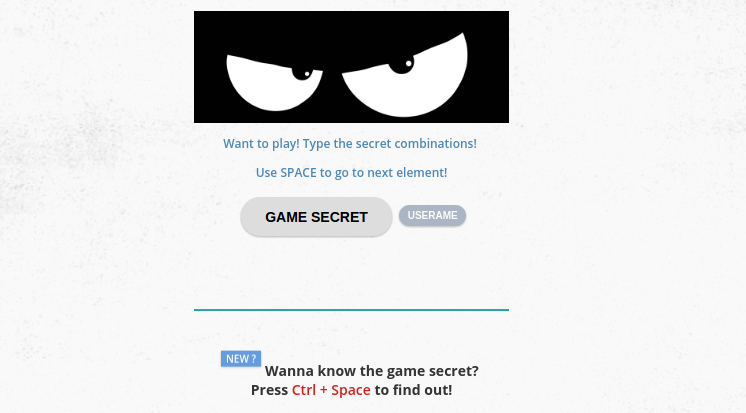
\includegraphics[width=\linewidth]{figures/experiment2/startscreen-game.png}
  \caption{The game start screen presented to player when entering the game for the first time}
  \label{fig:game-startscreen}
\end{figure}


The onboarding process starts by asking players to type the words that appear in the screen as small boxes. Points are awarded to the player regardless of their typing speed (rewarding and recognizing the players' effort). After the player is familiarized with the way the game works (typing fast while paying attention to the words that appear in the screen), the game continues by introducing a new challenge: a puzzle combined with typing skills. The puzzle consists of several hidden characters that the player has to reveal by typing the words appearing in the screen. The faster the typing the faster the revealing of characters. After the player has revealed all the characters on the puzzle, he is presented with a quiz where the \textit{question} is the revealed word (i.e. the named entity) and the options are the candidate entities extracted from \ac{kb}. Contextual clues are provided on top of the screen as sticky notes which help the player to make a correct decision. The quiz is a \textit{masked} version of the named entity disambiguation process used in the first experiment. The player proceeds by selecting a candidate option which is rewarded with 10 game points. Please note that if the player selects the wrong option, the system will not proceed until the right option is selected. As a reward for choosing the correct answer, the player finally reaches the end of the trial process where the game secret is finally revealed. Additionally, the player has to register himself with authentication credentials which together with the game secret are used as a secret combination for granting access to the game. Figures \ref{fig:onboarding}(a) to  \ref{fig:onboarding}(f) illustrate the complete onboarding process of Fastype. 

\begin{figure}[]
  \centering
  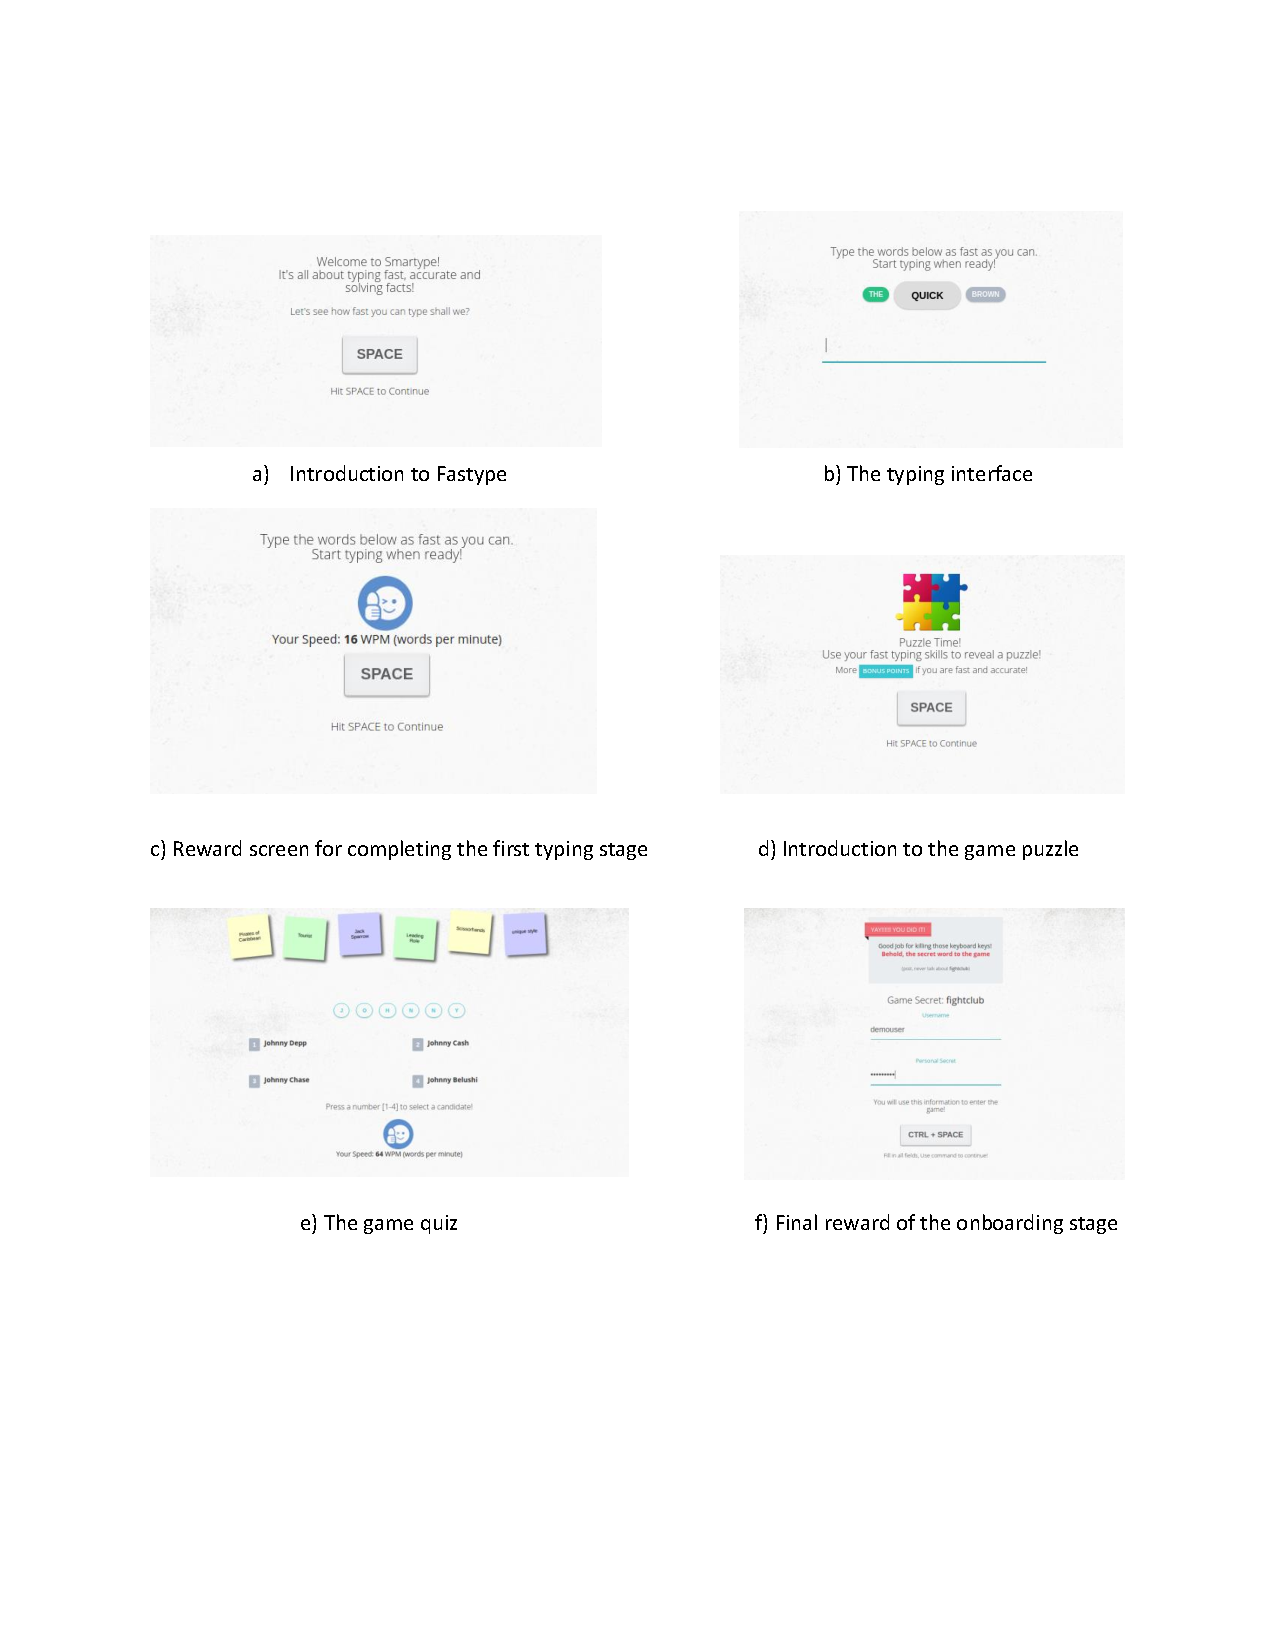
\includegraphics[page=1,width=\textwidth]{figures/experiment2/oboarding.pdf}
  \caption{The onboarding stage of Fastype}
  \label{fig:onboarding}
\end{figure}